% For tracking purposes - this is V2.0 - May 2012

\documentclass{sig-alternate-05-2015}

\usepackage[utf8]{inputenc}

%remove copyright
\makeatletter
\def\@copyrightspace{\relax}
\makeatother

\begin{document}

% Copyright
\setcopyright{acmcopyright}

% DOI
\doi{10.475/123_4}

% ISBN
\isbn{123-4567-24-567/08/06}

%Conference
\conferenceinfo{PLDI '13}{June 16--19, 2013, Seattle, WA, USA}

\acmPrice{\$15.00}

%
% --- Author Metadata here ---
\conferenceinfo{WebMedia}{'16 Teresina, Piauí Brazil}
%\CopyrightYear{2007} % Allows default copyright year (20XX) to be over-ridden - IF NEED BE.
%\crdata{0-12345-67-8/90/01}  % Allows default copyright data (0-89791-88-6/97/05) to be over-ridden - IF NEED BE.
% --- End of Author Metadata ---

\title{LiveSync: a Tool for Real Time Video Streaming Synchronization from Independent Sources}

\numberofauthors{3} %  in this sample file, there are a *total*
% of EIGHT authors. SIX appear on the 'first-page' (for formatting
% reasons) and the remaining two appear in the \additionalauthors section.
%
\author{
% You can go ahead and credit any number of authors here,
% 1st. author
\alignauthor
		Marcello N. de Amorim\\
       \affaddr{UFES}\\
       \affaddr{Av. Fernando Ferrari, 514}\\
       \affaddr{Vitória - ES, Brazil}\\
       \email{novaes@inf.ufes.br}
% 2nd. author
\alignauthor
		Ricardo M. C. Segundo\\
       \affaddr{UFES}\\
       \affaddr{Av. Fernando Ferrari, 514}\\
       \affaddr{Vitória - ES, Brazil}\\
       \email{rmcs87@gmail.com}
% 3rd. author
\alignauthor 
		Celso A. S. Santos\\
       \affaddr{UFES}\\
       \affaddr{Av. Fernando Ferrari, 514}\\
       \affaddr{Vitória - ES, Brazil}\\
       \email{saibel@inf.ufes.br}
}
\date{11 August 2016}

\maketitle
\begin{abstract}
	This work presents a tool that allows users to synchronize live videos from multiple sources such as YouTube or any other video streaming sources. The proposed approach to proceed the multiple camera video synchronization is based in crowdsourcing techniques, using the power of a crowd of collaborators to synchronize videos, requiring from each user the sync of only a pairs of videos. Additional sync relations are inferred from the known contributions, using transitivity properties and an appropriate structure for this inference, the Dynamic Alignment List.  
\end{abstract}


%
% The code below should be generated by the tool at
% http://dl.acm.org/ccs.cfm
% Please copy and paste the code instead of the example below. 
%
 \begin{CCSXML}
<ccs2012>
	<concept>
		<concept_id>10002951.10003260.10003282.10003296</concept_id>
		<concept_desc>Information systems~Crowdsourcing</concept_desc>
		<concept_significance>500</concept_significance>
	</concept>
	<concept>
		<concept_id>10003120.10003130.10003233.10011765</concept_id>
		<concept_desc>Human-centered computing~Synchronous editors</concept_desc>
		<concept_significance>500</concept_significance>
	</concept>
</ccs2012>
\end{CCSXML}

\ccsdesc[500]{Information systems~Crowdsourcing}
\ccsdesc[500]{Human-centered computing~Synchronous editors}

\printccsdesc

\keywords{live video; synchronization; crowdsourcing}

%%%%%%%%%%%%
%Introdução%
%%%%%%%%%%%%
\section{Introduction}
Multiple camera video synchronization is a research area within multimedia. Automatic video synchronization (AVS) is a form to synchronize multiple video streams. AVS can be done analysing video segments \cite{wang2014videosnapping} or audio ones \cite{su2012making}. In Schweiger et.al.\cite{schweiger2013fully} we find these and other approaches in the area. One main contribution of this paper is the description of the challenges for automatic synchronization algorithms: wide baselines, camera motion, dynamic backgrounds and Occlusions.

We propose in this work the use of crowdosurcing techniques to synchronize these videos, instead of an automatic one. Crowdsourcing \cite{howe2006rise} in our scope refers to the use of the crowd as part of a computational problem that can be solved easily by a human than by a machine. The "easily" word can mean that the human approach: is cheaper, faster or can be done more efficiently by humans.

In video synchronization, we know that humans can fulfil all challenges presented by \cite{schweiger2013fully}. A person can identify if two videos are synchronized or not independently of occlusions, change of the background, camera motion or view point changes. The main challenge is how to use the human abilities to synchronize the videos, and permit that other persons can benefit from these contributions. So our tool uses the power of the crowd to synchronize live streaming videos and provide a form that other persons that want to watch those videos can receive both videos and synchronization info.

The remaining of this paper is presented as follows: section 2 explains our approach to synchronize videos; section 3 details our tool; and section 4 presents our final remarks.

%Dinamic Aligment List%
\subsection{D.A.L.}
To synchronize the video streams we use an synchronization technique presented in \cite{segundo2015remote}: the Remote Temporal Couplers for aligning videos. It allows us to synchronize independent videos from multiple sources and to infer unknown relations from videos. We implemented the technique under our Dynamic Alignment List structure.

A DAL derivates from a matrix m x n, with m and n natural numbers, where m=n is the quantity of videos that can be synchronized at that moment. Each position of the matrix represents the relation of two videos (the coupler), in other words, the value necessary to align them, in our synchronization scenario. This value is calculated using: $\Delta_{i,j}=begin(id_{i,0})-begin(id_{0,j}), para 0<i,j\neq m $, where begin(x) is the time where an asset X begins its presentation. A $\Delta_{i,j} > 0$, implies that the asset in the column starts $\Delta_{i,j}$ before the asset in the line. Case $\Delta_{i,j} < 0$, the opposite happens and case $Delta_{i,j} = 0$, both starts at the same time.

As previously said, the list is derived from a matrix, presenting different aspects. Firstly, it does not presents all cells of a matrix. In the matrix, $\Delta_{i,j}$ is equal to $\-Delta_{j,i}$, so we don't need to store both relations, and with that, only the superior part of the relations are stored. Secondly, each "cell" of the list, presents multiple properties to help in the management of the crowd contributions. As each relation can contain multiple contributions, we need to calculate a mean of these contributions  to set as the actual $\Delta$. Lastly, each relation has a new dimension: a list with all contributions for that relation, that identifies the value of the contribution and the user that made it (if we want to identify who made it).

Figure~\ref{dal}, shows the representation of a DAL. There we have 5 assets (videos in our scope) labelled: A, B, C, D and E. Each asset represents a struct with the assets: URI, label, duration and a list of relations with the other assets. Following the asset A we find its relations with the other assets: AB, AC, AD and AE. We do not need to represent AA because $\Delta_{A,A}$ is always 0. Taking teh relations from B, we have: BC, BD and BE.  Again, $\Delta_{B,B} = 0$. Thus, we do not represent BA, because we previously represented AB, and as said before, we can find BA by negating AB ($\Delta_{A,B} = -\Delta_{A,B}$). And this will happens to the other relations.

In the end of the DAL, we have the contributions for each asset (represented in the figure by a cloud due to figure dimensions). Each relation can receive multiple contributions, and are stored in the list. These contributions are processed (means) and generate the value of $\Delta$ for its relations. Fields such as confidence factor and number of contributions are used to know how robust those contributions are, and if its necessary more contributions to verify the synchronization.

\begin{figure}
	\centering
	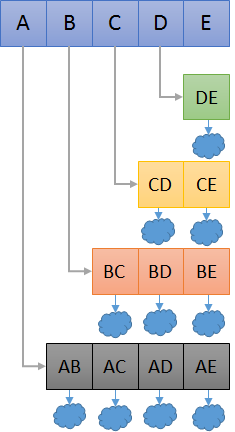
\includegraphics[scale=0.4]{figure/dal}
	\caption{DAL with 5 Assets (A,B,C,D,E)}
	\label{dal}
\end{figure}

%%%%%%%%%%%%%%%%%%%%%%%%%%%
%LiveSyncDescription/Metas%
%%%%%%%%%%%%%%%%%%%%%%%%%%%
\section{LiveSync}
Live synchronization includes the scenario where a viewer has access to an event that is live streamed by more than one Content Provider. These content providers are independent, so their videos do not have initial resources that allow their automatic synchronization to viewers, requiring a video analysis to generate synchronization points (Couplers). This synchronization fits as a problem that can be solved by using the power of the crowd. This occurs because videos are generated independently, without synchronization points and without previous description of what is about to be shown in screen, neither how can it be correlated to other videos. This way, human perception is used in real time to generate unknown synchronization points. 

As example for this scenario, we can take a public manifestation. In the event, multiple people can take their cell phones and start streaming the event. In their house, other people can watch the videos. However, the multiple videos from different sources will be asynchronous. We need a way to synchronize these UGV. We use the crowd to achieve it. To this objective we group all videos in a MashUp application that connects to a Coupler Server that contains all synchronization data. Both synchronizing and playing the videos are made using this mashup, that can receive videos from multiple sources.

\subsection{Method}
In a live presentation, it is assumed that content must be consumed right after its generation. It is of extreme importance that the synchronization method can be performed in playback time, to allow the integration of live content.

The way synchronization is performed in live video poses a single requirement: in a live situation, there is no need to analyse an entire video to find synchronization points, only an estimated stream delay must be considered. This occurs because the event is happening in real time (live), sources are also live and, therefore, the lack of synchronization during playback is caused by video streaming delays. In this specific case, synchronization through the crowd may be achieved by using tools that allow a user to manipulate time from videos: he can, for instance, keep pausing videos alternately , until he feels they are synchronized. This is a consequence of having a reduced search space, when limited to stream delays between videos.

However, not all viewers are required to be part of the crowd to achieve synchronization. If a synchronization made by a single member of the crowd is accepted as accurate, it can be transferred to the remaining viewers, this way each one will have his content locally synchronized.

One way of live synchronization can work is as follows: a person selects and synchronizes two videos with the help of a manipulation tool. This becomes a candidate synchronization point. Several people can do the same, and the results can be based on multiple synchronizations. Having these synchronization points defined, synchronization information can be sent to other viewers interested in watching those videos. As simple example, take two independent sources that are transmitting an event. A mash-up system allows the user to watch both videos at the same time is his device. However the videos are asynchronous and the user notes that. He then access the option to synchronize the videos. After he achieve a synchronous result, implicitly his contribution is sent to a server that will feed other users that choose to watch the same videos with the synchronization specification. If the user thinks the content is not synchronised yet, he can synchronize it himself and send another contribution.

%Funcionalidades%
\subsection{Main Functionalities}
	The main functionalities provided by our tool are:

\textbf{\textit{Synchronized Live Video Player:}} The tool permits users to watch multiple videos synchronized. He selects from a list of sources the videos he wishes to watch and them they are synchronized using information provided by other users.

\textbf{\textit{:}} If a pair of videos does not have any information about their synchronization, users are invited to contribute and synchronize the videos.

\textbf{\textit{Synchronization Infering:}}	
	In some cases that there is no direct information about the synchronization of two videos, the tool is able to infer the synchronization about them, based on the contributions of other videos. We use the transitive attribute of video synchronizations, where if we know AB and BC synchronization info (couplers), we can infer AC. To infer this value we travel trough the DAL, finding the unknown relations (for example, CE), and try to find a path of known relations where we can infer CE. Taking the DAL in Figure~\ref{dal}, we can infer CE if we know: AC and AE. This a two steps route, but we try all possible routes when inferring, in a way that we fill as much relations as possible.
	
\textbf{\textit{Video Aggregation:}} Although the focus of the LiveSync tool is on synchronization, we allow users to add new stream sources to the application. He only needs to set the video source, and the video will be added to the DAL and list of videos. However, we don't do any filtering about the added video, this means that the user can add any video to the application, even ones that contains none relation with the other videos. In future versions we plan to add options where other users can mark the video as not related, and then remove them.
	
\textbf{\textit{Multiple Platform Support:}} One keypoint of our tool is the use of other platforms as video sources. The videos that we play to users and that are synchronized, are not provided by us, but by other live video stream platforms. To be compatible with our tool, two requisites are required:
	\begin{enumerate}
		\item Remote Player: we need that the platform allows embeddable players on third pages, allowing us to control the player with its basic functionalities such as: play, pause and stop;
		\item Uptime Support: a second and fundamental requisite is an API that allows us to retrieve the video Uptime. Video uptime is the time since the beginning of the video that is presented on the video player. This is fundamental to create and replicate the couplers generated in synchronization process.
	\end{enumerate}

\textbf{\textit{Serverless Architecture:}} Serverless architectures refer to applications that significantly depend on third-party services and putting much of the application behavior and logic on the front end. Such architectures remove the need for the traditional server system sitting behind an application \cite{RobertServerless}. More of this characteristic will be addressed in the next topic: Architecture.

\textbf{\textit{Multiplatform:}} LiveSync is a Web Based application designed and developed in compatibility with HTML5 standard to its front-end (MashUp Player) component. It allows our application to run on multiple browsers, operational systems and devices.

\textbf{\textit{Active X Passive Contributions:}} Two branches of the LiveSync are currently on our repositories. They differ only in one aspect: who defines what videos are to be synchronized: the crowd or the application? The active version allow users to navigate freely through the videos, synchronizing them when they wish to. The focus of this branch is to allow users to contribute if they want to. On the other hand, in the Passive branch the server gives the crowd exactly what video they will synchronize. The focus here is to rapidly synchronize all videos, so the focus isn't to make users watch the videos, but force them to synchronize all the base for other porpoises. The active branch is the focus here, but can easily converted to the passive one.

%Arquitetura%
\subsection{Architecture}
The LiveSync tool has three main components (Figure~\ref{livesync}): the Content Providers (Video Sources), the Coupler and the Mashup Player.

\begin{figure}
	\centerline{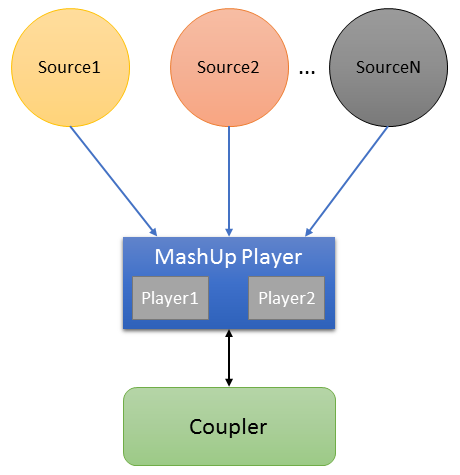
\includegraphics[scale=0.4] {figure/arqchitecture}}
	\caption{Modelo simplificado do live-sync}
	\label{livesync}
\end{figure}

\subsubsection{Content Providers}
Content Providers are third-parties videos streamers platforms. There are multiple Live Video Stream applications in the market, such as YouTube Live, LiveStream, TwitCast, Twitch and Ustream. One of our objective was to allow the use of different platforms as video sources, so we maximize the number of videos for an event and allow the use of already in market platforms. 

A Content Provider needs two requisites to be compatible with LiveSync: a Remote Player and Uptime Support. As each stream platform uses their own protocols, we opt to use their embeddable players into a MashUp application. These players must allow us to play, pause and stop the video stream. The second requisite, Uptime Support, is necessary to find the couplers among the videos. Uptime is the time passed since the beginning of the live stream until the video part being presented in the player at the moment of the call.

At this time, LiveSync supports two video stream platforms: the YouTube Live (https://goo.gl/DEM9eW) and WebSocket Stream (http://goo.gl/GYnGpg). YouTube live allows live stream from both desktop and mobile devices, making possible users to stream any event they wish with low effort: they only need to install the software and to have a YouTbe account. WebSocket Stream is an open source project that allows developers to implement live stream services with websockets and canvas and WebGl technologies. It works in any browser and was used for our first tests where we needed full control of the stream, something that YouTube Live doesn't support.

To add an video source form a Content Provider, it necessary only the video ID from YouTube Live or the video stream URI from the WebSocket Stream. These are added as assets to the LiveSync and can be accessed or synchronized.

\subsubsection{Coupler}
The Coupler is responsible for storage, distribution and calculation of synchronization points among video streams from the Content Providers.

A coupler is composed of a DAL instance and Log files. This goes in direction of the Serverless Architecture. We wanted an architecture that needed low resources (another justification for using third party stream services) and easy deployment. All that is necessary do execute the coupler is a NODE.JS (https://nodejs.org/en/) server instance. This is possible because the Coupler is fully developed in JavaScript and compatible with the HTML5 standards. To deploy the Coupler, we use a Backend as a Service or "BaaS" platform, more specifically we use the Heroku (www.heroku.com) one, that permits free use of NODE.JS instances.

It stores synchronization information only during the duration of the event, so its stance is finished with the end of the videos and all data is lost. In the current scope, the sync info is only necessary during the event, after it, there is no need to store the information. For reasons of testing and using the filmed videos from YouTube we create log files that contains all contributions made by the crowd. If it is important to maintain all contributions and data for post analyses and further use, unstable version of the LiveSync is being configured to use a fully transactional database. We use a fully transactional database because we want to maintain track of all contributions made by the crowd, an important aspect in crowdsourcing and that is also supported by the DAL.

Other aspect of the Coupler is that it is responsible for the distribution of synchronization couplers. When a user chooses two videos, a message is sent from the MashUp to the coupler, containing the required relation. The coupler then answer with the required information. If the relations is unknown, it answer soliciting the user to synchronize and contribute with those two videos.

The last function of the Coupler, is to calculate the synchronization points among Videos. Each relation ($\Delta_{A,B}$) may contain several contributions, then it is necessary to calculate a value to that relation based on the contributions. In the current version we calculate a Geometric Mean of the contributions to find an ideal value. This however may not be the best value, because the more accurate the sync is, the better the results are, so older contributions must have a lighter weight, something that does not happen in current version. The other calculation made by the coupler, is to infer unknown relations based on the afore mentioned transitive relation.

The communication  between Coupler and MashUp is made through Websocket communication. The MashUp creates a WebSocket channel with the Coupler, and requests the sync information or sends contributions from the crowd. A simple protocol is used in JSON messages: {act:value, data:object}. The act field contains the action to be made and the data contains an object to complement the action. As example we have an act to send a new contribution ("contribution") that is complemented with a new relation that contains the assets involved, the value and an id to that contribution.

\subsubsection{MashUp Player}
Mashups are applications generated by combining content, presentation or other applications functionalities from disparate sources. They aim to combine these sources to create useful new applications or services (the offer and consumption of data between two devices) to users \cite{yu2008understanding}. In LiveSync we combine videos coming from different sources and platforms with the synchronization information from the coupler to reproduce a synchronous presentation of these videos.

The MashUp Player (Figure 3) is responsible for both presenting video synchronously and collecting the synchronization. Figure~\ref{screen1} represents the interface of the MashUp.

\begin{figure}
	\centerline{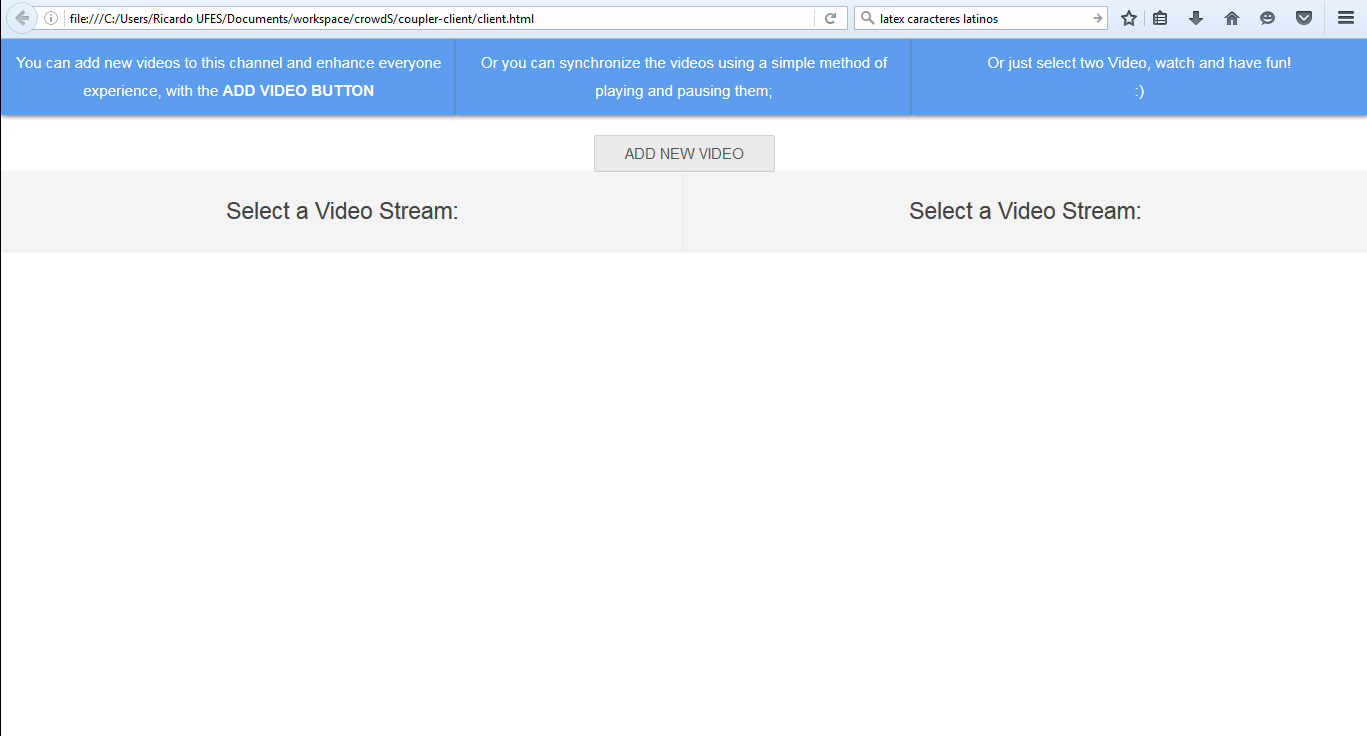
\includegraphics[scale=0.17] {figure/screen}}
	\caption{Modelo simplificado do live-sync}
	\label{screen1}
\end{figure}

On the top we have all information necessary to the user. He can aggregate new videos using the ADD NEW VIDEO options, SYNCHRONIZE the videos if he thinks the videos are not synchronized or he can just select the videos he want to watch. When just playing two selected videos from the videos list, each video player creates an instance for the player that is compatible with that source (YouTube or WebSocket). It is invisible to the user where the video is coming from.

When the user adds a video, an input text is shown to him, and he can add the video URI (WebSocket) or video ID (YouTube). The page reloads and the new video is listed in the video list for everyone that connects to the application. When the video is added by the user, an message is sent to the Coupler, containing the action to add a new asset to the DAL, and the specification of it, such as label and URI.

The last functionality of the MashUp is to synchronize the videos. When the user clicks on SYNCHRONIZE, a new mode of the application is revelled showing the synchronization tools. We use a Play 'n Pause approach to synchronize the videos. After the user thinks the videos are synchronized, clicking the DONE button, his contribution is sent to the Coupler and stored in the DAL for further processing of the relation.

\textbf{\textit{Play 'n Pause:}} If two videos with a certain degree of similarity, are presented to an individual from the crowd, he can possibly notice that one video is ahead of the other. This way, he can pause the video that is ahead on time while the other remains playing, until reaching a point of synchronization. Then, the user can resume playback of the first video. This process can be repeated until an individual feels like both videos are being presented synchronously. On [https://goo.gl/HTzecL], readers can see the play and pause technique being used to synchronize two live streams from from Two YouTube servers.

\section{Final Remarks}
The LiveSync tool allows users to watch live video streams from multiple sources synchronized. If the videos are not synchronized, user can contribute and synchronize themselves the videos and help building the synchronization, in a crowdsourced approach, believing that using human perception is better than using automatic approaches in this specific case.

Our tool however presents some limitations that shall in the futures be suppressed, such as the number of events that we can follow. Now, each instance of Coupler and MashUps can handle only one event, in other words, we can't cover two independent live events at the same time with one instance, for that porpoise we need more than on instance of each service. Also, new stream services must be added to increase our compatibilities.

Within this work publication, the code will be made public through a GitHub repository under a Common Core License.

%ACKNOWLEDGMENTS are optional
%\section{Acknowledgments}
%The authors would like to thank the "Fundação de Amparo à Pesquisa e Inovação do Espírito Santo" (FAPES) for financial support.

\bibliographystyle{abbrv}
\bibliography{sigproc}  
\end{document}
